\documentclass[a4paper,12pt]{report}

\usepackage{alltt, fancyvrb, url}
\usepackage{graphicx}
\usepackage[utf8]{inputenc}
\usepackage{float}
\usepackage{xcolor}
\usepackage{hyperref}

% Questo commentalo se vuoi scrivere in inglese.
\usepackage[italian]{babel}

\usepackage[italian]{cleveref}

\title{Elaborato per il corso di\\''Programmazione di Reti''}
\author{Rebosio Alessandro}
\date{\today}

\begin{document}

\maketitle

\tableofcontents

\chapter{Introduzione}

L'obiettivo di questo progetto è la realizzazione di un \textbf{server HTTP} \newline minimale sviluppato in \textbf{Python},
capace di gestire richieste di tipo \texttt{GET} sulla \texttt{porta 8080} di localhost e di servire contenuti statici
in formato HTML e CSS.

\vspace{0.5cm}

\noindent Il progetto intende fornire una comprensione pratica del \textbf{protocollo \newline HTTP}, dell'utilizzo dei \texttt{socket}
per la comunicazione di rete e del funzionamento di base di un \texttt{web server}.

\subsubsection{Funzionalità principali}
\begin{itemize}
    \item Risposta con codice di stato 200 per risorse esistenti;
    \item Gestione dell'errore 404 per risorse non trovate;
    \item Riconoscimento e gestione dei MIME types per i file serviti;
    \item Logging delle richieste ricevute;
    \item Pubblicazione di un sito web statico composto da tre pagine HTML responsive.
\end{itemize}


\chapter{Archittetura del progetto}
L'architettura del progetto si basa su una \texttt{suddivisione} tra la logica \newline applicativa del server e i
contenuti statici da servire al client.

\section{Descrizione dell'architettura}
\begin{itemize}
    \item \textbf{src/server.py}: implementa il web server HTTP, ascolta sulla porta 8080 e serve file
          statici presenti nella cartella \texttt{www/}.
    \item \textbf{www/}: contiene il sito web statico, costituito da tre pagine HTML e un file CSS
          condiviso. Le pagine includono layout responsive e contenuti base.
\end{itemize}

\begin{figure}[H]
    \centering
    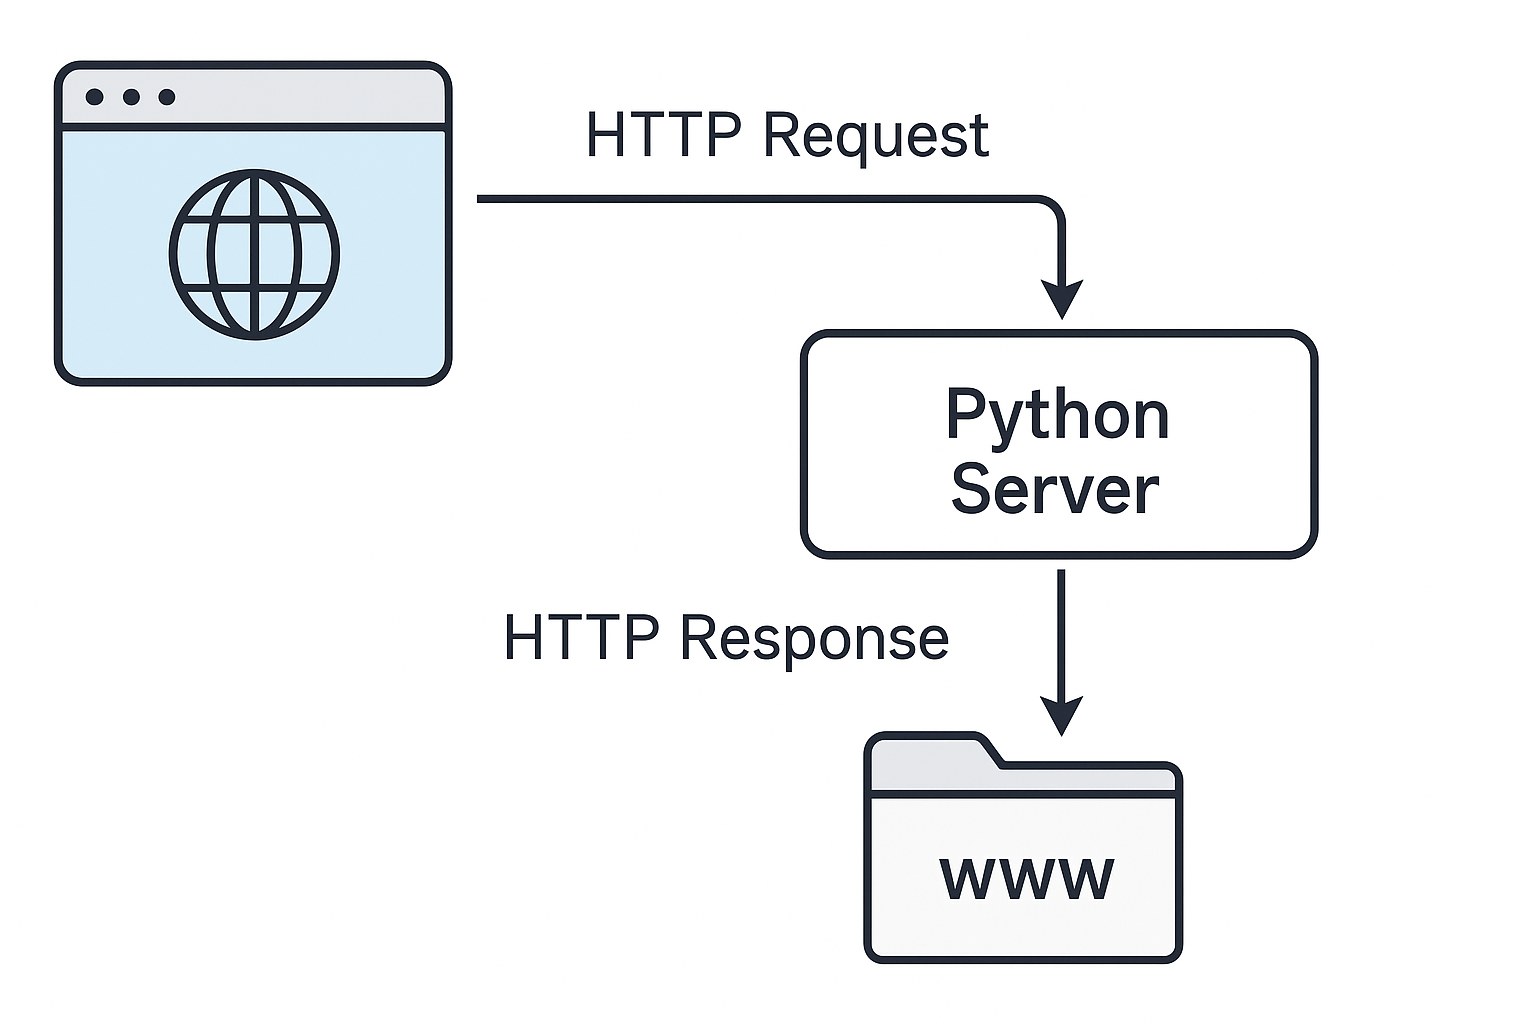
\includegraphics[width=0.5\textwidth]{img/architettura.png}
    \caption{Schema dell'architettura client-server}
    \label{fig:architettura}
\end{figure}

In \Cref{fig:architettura} viene rappresenta l'interazione tra browser, server e file system. Quando un client
invia una richiesta HTTP, il server interpreta la richiesta, individua il file richiesto nella directory \texttt{www/}
e restituisce il contenuto.


\chapter{Implementazione del web server}
L'implementazione del server HTTP è interamente in \texttt{Python} utilizzando il modulo \texttt{socket} per
la comunicazione e il modulo \texttt{threading} per la gestione concorrente delle connessioni.

\section{Struttura generale}
\begin{itemize}
    \item \textbf{HTTPServer}: classe usata per stabilire una o più connessioni \newline attraverso la creazione di
          un \texttt{socket}, che viene poi associato alla \texttt{porta 8080} per accettare le connessioni in ingresso.
    \item \textbf{HTTRequestHandler}: classe per il parsing delle richieste con il successivo invio di risposte.
    \item \textbf{MyServer}: sottoclasse per semplificare la logica, nella quale viene implementato il
          metodo \texttt{do\_GET} per servire i file richiesti dai client.
\end{itemize}


\section{Gestione delle richieste}
Quando un client tenta la connessione e viene accettata, il server crea un nuovo \texttt{thread} per gestirla, permettendo
le richieste in modo concorrente.

La richiesta viene letta, vengono estratti il \texttt{metodo}, \texttt{path} e la \texttt{versione HTTP} dalla prima
riga.

Successivamente se la risorsa richiesta esite nella directory \texttt{www/}, viene caricata e restituita la risposta
con il codice \texttt{(200, OK)}. Altrimenti viene restituita la risposta di errore con il codice \texttt{(404, Not Found)}.

\section{Gestione MIME types e logging}
Il server usa la libreria \texttt{mimestype} per determinare il tipo di contenuto da servire in base all'estensione del
file.

\vspace{0.5cm}

\noindent Ogni \texttt{richiesta} viene loggata \Cref{fig:logging} in console con il formato:

\begin{verbatim}
    ip  - - [data] "metodo risorsa versione" codice -
\end{verbatim}

\subsubsection{Esempi di logging:}
\begin{figure}[H]
    \centering
    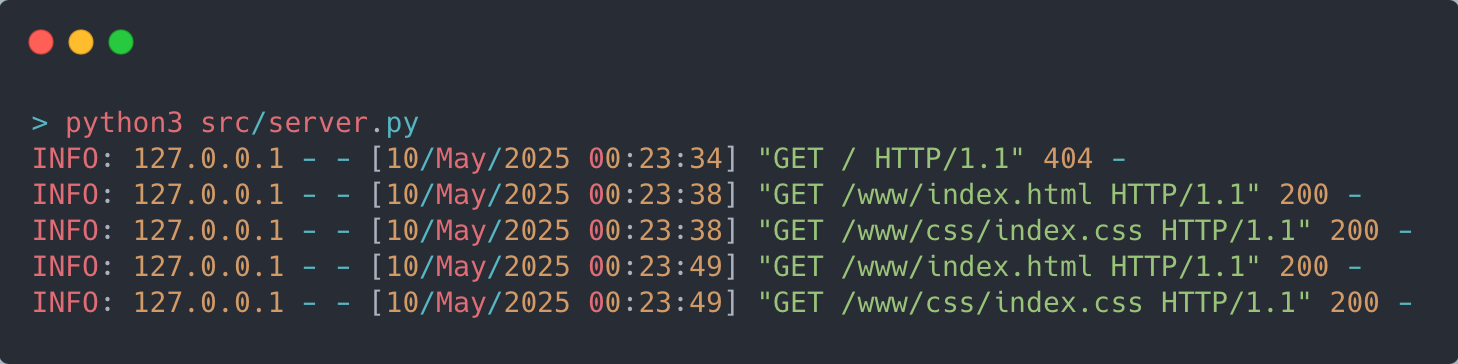
\includegraphics[width=1\textwidth]{img/logging.png}
    \caption{Log delle richieste in console}
    \label{fig:logging}
\end{figure}

\section{Sicurezza base}

Per evitare accessi non autorizzati a file esterni alla cartella \texttt{www/}, il \newline path richiesto viene sanificato
rimuovendo sequenze potenzialmente pericolose come \texttt{../}.

\subsubsection{Sicurezza del path:}
\begin{figure}[H]
    \centering
    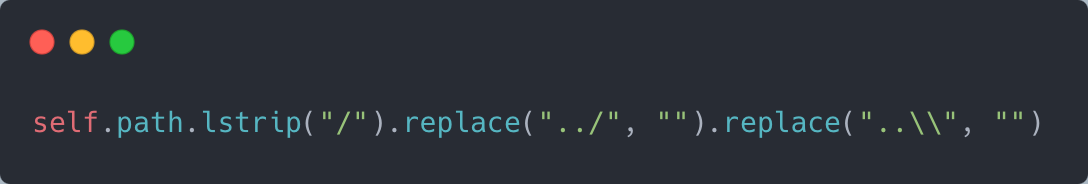
\includegraphics[width=1\textwidth]{img/safe_path.png}
    \caption{Codice per path sicura}
    \label{fig:safe_path}
\end{figure}


\chapter{Sito web statico}
Il sito web servito dal web server, al momento, è composto da tre pagine HTML statiche, con layout responsive e stile definito
tramite file CSS dedicati. L'obiettivo è fornire un'interfaccia semplice per dimostrare il corretto caricamento dei contenuti
da parte del server.

\section{Pagine HTML}

\begin{itemize}
    \item \textbf{index.html} - Homepage che presenta una navigazione verso le altre sezioni del sito.
    \item \textbf{login.html} — Simula una pagina di login: nel caso venga inviata una richiesta POST, il server restituirà un errore 501 (metodo non implementato).
    \item \textbf{contact.html} — Pagina di contatto, con pulsanti per tornare alla home o alla pagina di login.
\end{itemize}
%
\textit{Tutte le pagine fanno uso del framework \texttt{Bootstrap 5} per garantire un design responsive e compatibile con dispositivi di varie dimensioni.}

\section{Estendibilità}

Il sistema è progettato per essere facilmente estendibile: per aggiungere una nuova pagina è sufficiente \texttt{creare} un file HTML nella cartella
\texttt{www/} e assicurarsi che il \texttt{collegamento} nel sito punti al percorso corretto.

\begin{quote}
    \textit{Non è necessario modificare il codice del web server: qualsiasi file esistente sarà automaticamente servito, a condizione che venga effettuata una richiesta HTTP valida.}
\end{quote}


\chapter{Test e risultati}
Al fine di verificare il corretto funzionamento del web server, sono stati condotti diversi test utilizzando lo strumento da linea di comando \texttt{curl}, utile per simulare
richieste HTTP verso il server.

\section{Test funzionali}
\subsection{Richieste valide (200 OK)}
Sono state effettuate richieste HTTP di tipo \texttt{GET} verso le pagine HTML presenti nella cartella \texttt{www/}.

\begin{verbatim}
curl -i http://localhost:8080/www/index.html
\end{verbatim}

\textbf{Risposta:}
\begin{verbatim}
HTTP/1.1 200 OK
Content-Type: text/html
Content-Length: 872
\end{verbatim}

\begin{itemize}
    \item \url{http://localhost:8080/www/index.html}
\end{itemize}
La stessa risorsa è accessibile anche da un browser web digitando l'URL nella barra degli indirizzi, a condizione che il server sia attivo in locale sulla porta \texttt{8080}.

\newpage
\subsection{Risorse non trovate (404 Not Found)}
È stata verificata la gestione degli errori accedendo a una risorsa non presente nella cartella \texttt{www/}. Il server ha risposto correttamente con un errore \textbf{404 Not Found}.
\begin{verbatim}
curl -i http://localhost:8080/www/missing.html
\end{verbatim}

\textbf{Risposta:}
\begin{verbatim}
HTTP/1.1 404 Not Found
Content-Type: text/html
Content-Length: 1245
\end{verbatim}

\begin{itemize}
    \item \url{http://localhost:8080/www/missing.html}
\end{itemize}
La stessa richiesta, effettuata tramite browser, produce una pagina di errore ben formattata, confermando la corretta gestione dell'errore da parte del server.

\subsection{Metodo non supportato (501 Not Implemented)}
È stata testata la risposta del server a una richiesta POST verso la pagina di login:
\begin{verbatim}
curl -i -X POST http://localhost:8080/www/login.html
\end{verbatim}

\textbf{Risposta:}
\begin{verbatim}
HTTP/1.1 501 Not Implemented
Content-Type: text/html
Content-Length: 567
\end{verbatim}

\begin{itemize}
    \item \url{http://localhost:8080/www/login.html}
\end{itemize}
Lo stesso comportamento può essere osservato tramite browser, quando si tenta di inviare il form di login.

\vspace{0.5cm}

\begin{quote}
    \textit{Questo risultato è coerente con le specifiche del progetto, che prevedono l'implementazione solo del metodo GET per
        la gestione di richieste HTTP.}
\end{quote}

\subsection{Test sui MIME types}
Il server ha correttamente identificato il tipo di MIME dei file richiesti:
\begin{itemize}
    \item \texttt{.html} $\rightarrow$ \texttt{text/html}
    \item \texttt{.css} $\rightarrow$ \texttt{text/css}
    \item \texttt{.jpg}, \texttt{.png} $\rightarrow$ \texttt{image/jpeg}, \texttt{image/png}
\end{itemize}

\subsection{Conclusioni dei test}
Tutti i test funzionali hanno confermato la robustezza del server nell'ambito dei requisiti minimi. Le estensioni implementate (gestione MIME, logging)
hanno migliorato l'usabilità e la compatibilità con i browser moderni. La struttura modulare facilita inoltre futuri ampliamenti.


\chapter{Conclusioni}
Il progetto ha raggiunto tutti gli obiettivi prefissati, realizzando un web server HTTP minimale ma funzionale in Python. Attraverso questo sviluppo sono stati approfonditi diversi aspetti fondamentali:
\begin{itemize}
    \item Il funzionamento del protocollo HTTP/1.1
    \item La gestione delle connessioni tramite socket
    \item L'elaborazione delle richieste e la costruzione delle risposte
    \item La gestione concorrente delle connessioni
    \item La sicurezza di base nell'accesso alle risorse
\end{itemize}

Il server sviluppato, pur nella sua semplicità, dimostra di essere in grado di gestire correttamente le richieste GET per file statici, con appropriate risposte di errore per risorse non trovate o metodi non implementati. L'integrazione con un sito web reale, seppur minimale, ha permesso di verificare il corretto funzionamento in uno scenario pratico.

\section{Sviluppi futuri}
Possibili estensioni e miglioramenti includono:
\begin{itemize}
    \item Implementazione del metodo POST per form interattivi
    \item Supporto per l'upload di file
    \item Aggiunta di un sistema di caching
    \item Implementazione di HTTPS per comunicazioni sicure
    \item Supporto per CGI o interfacce con linguaggi server-side
\end{itemize}


\end{document}
